\documentclass[letterpaper,11pt]{article}
\usepackage{cmap}
\usepackage[T1]{fontenc}
\usepackage[margin=0.75in]{geometry}
\usepackage{amsmath,amssymb}
\usepackage{graphicx}
\usepackage{booktabs}
\usepackage{longtable}
\usepackage{float}
\usepackage{setspace}
\usepackage{ragged2e}
\usepackage[numbers,sort&compress]{natbib}
\usepackage{hyperref}
\hypersetup{colorlinks=true,allcolors=black}
\usepackage{etoolbox}
\usepackage{xcolor}
\usepackage{soul}
\usepackage{caption}
\usepackage{authblk}
\usepackage{titlesec}
\usepackage[left,modulo]{lineno}
\usepackage{textcomp}
\usepackage{upgreek}
% Labels: \(\upalpha\) helix, C\(\upalpha\); variables: \(\chi_1\).

\captionsetup{font=normalsize,justification=justified}
\onehalfspacing
% Left-aligned body text, retaining the article first-line indentation.
\setlength{\RaggedRightParindent}{\parindent}
\AtBeginDocument{\RaggedRight}

\setcounter{secnumdepth}{3}
\titleformat{\section}{\normalfont\bfseries\normalsize}{}{0pt}{}
\titleformat{\subsection}{\normalfont\bfseries\normalsize}{}{0pt}{}
\titleformat{\subsubsection}{\normalfont\bfseries\normalsize}{}{0pt}{}
\renewcommand{\Authfont}{\normalfont\normalsize}
\renewcommand{\Affilfont}{\normalfont\normalsize}

\title{Supplementary Information: Scientific Manuscript Template Demonstration}
\author[1]{First Author}
\author[2]{Second Author}
\author[1,*]{Corresponding Author}
\affil[1]{Department of Example Studies, Example University, City, Country}
\affil[2]{Institute of Demonstration Research, Example University, City, Country}
\date{*Correspondence: author@example.edu}

\begin{document}
\modulolinenumbers[1]
\linenumbers
\maketitle

\renewcommand{\thefigure}{S\arabic{figure}}
\setcounter{figure}{0}
\renewcommand{\thetable}{S\arabic{table}}
\setcounter{table}{0}

\section{Supplementary Results}

The supplementary document provides extended datasets, control experiments, and sensitivity analyses that complement the main text \cite{sample2024}. 

\subsection{Supplementary Figure Demonstration}
Supplementary figures follow the shared asset conventions with a separate supplementary figure folder, utilizing the \texttt{../assets/figures/supplementary/} directory. Figure numbering automatically prefixes an ``S'' according to the document rules, as illustrated in Figure~\ref{fig:supp-example}.

\begin{figure}[htbp]
  \centering
  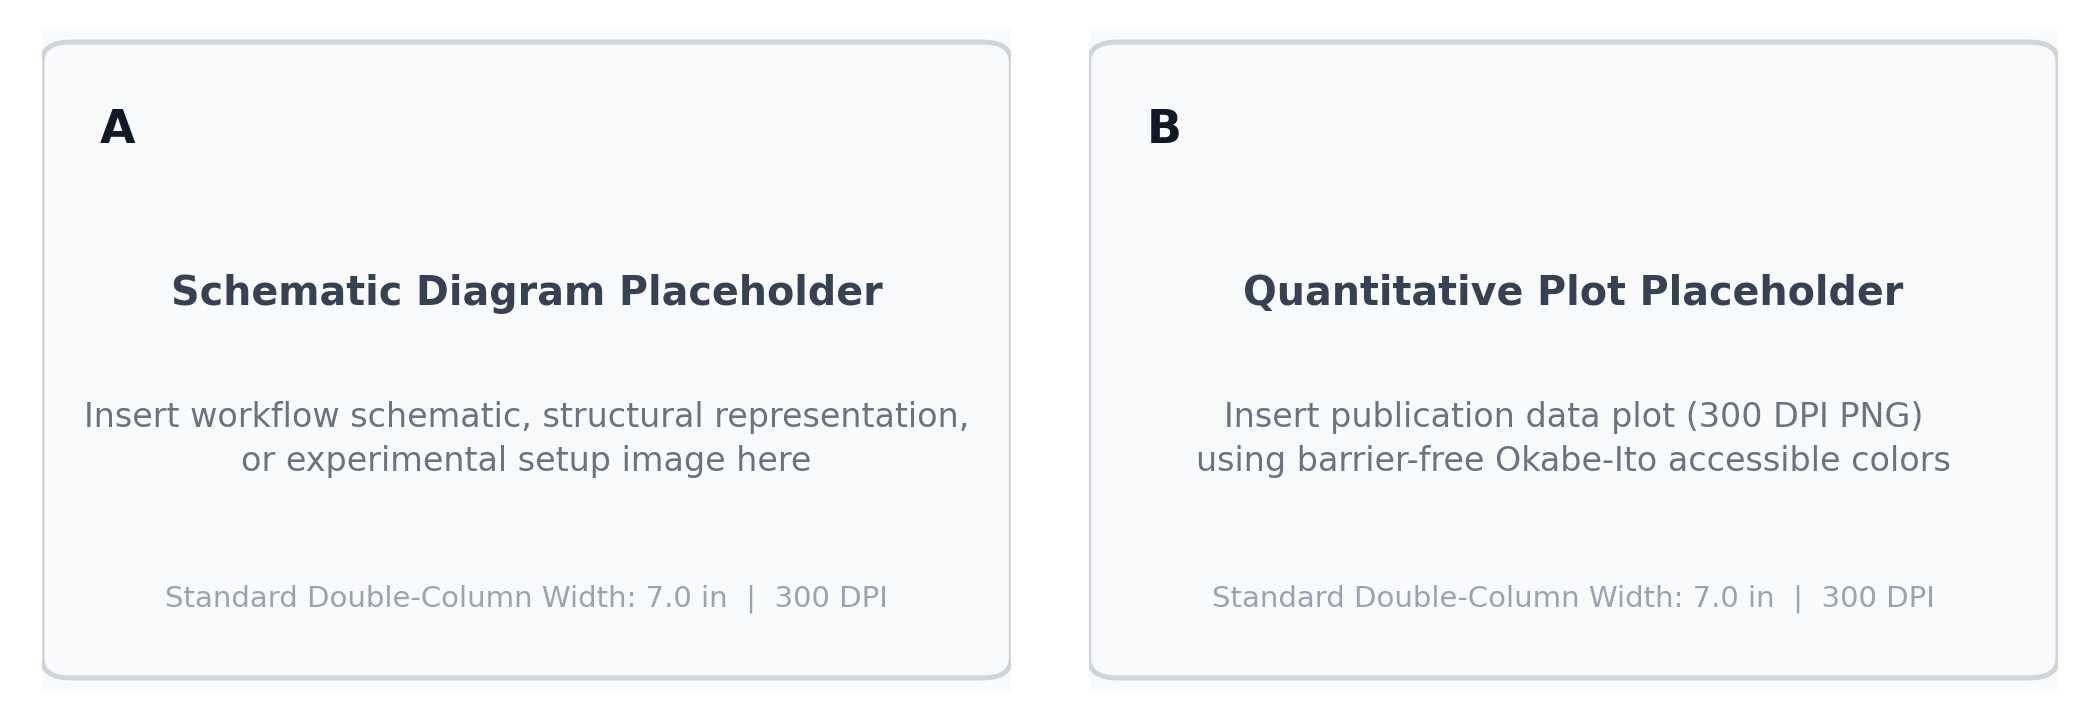
\includegraphics[width=\textwidth,keepaspectratio]{../assets/figures/supplementary/figure1.png}
  \caption{\textbf{Supplementary multi-panel figure placeholder.} 
  \textbf{(A)} Placeholder for extended control schematics or supplementary protocols. 
  \textbf{(B)} Placeholder for supplementary data plots and sensitivity analyses.}
  \label{fig:supp-example}
\end{figure}

\subsection{Supplementary Tabular Data}
Detailed workbooks, raw measurement tables, and extended data matrices are preserved under \texttt{../assets/tables/supplementary\_tables.xlsx}. Key summary subsets can be rendered directly using standard booktabs environments (Table~\ref{tab:supp-data}):

\begin{table}[htbp]
  \centering
  \caption{\textbf{Supplementary measurement parameters and validation summary.}}
  \label{tab:supp-data}
  \begin{tabular}{lcccc}
    \toprule
    \textbf{Sample ID} & \textbf{Condition} & \textbf{Measurement A} & \textbf{Measurement B} & \textbf{Status} \\
    \midrule
    SMP-01 & Control Baseline  & 10.5 & 1.25 & Pass \\
    SMP-02 & Treated Variant A & 20.1 & 2.50 & Pass \\
    SMP-03 & Treated Variant B & 35.8 & 4.10 & Review \\
    \bottomrule
  \end{tabular}
\end{table}

\section{Supplementary Methods}

\subsection{Detailed Protocols and Validation Steps}
This section documents step-by-step reproducibility details, hyperparameter specifications, and software environment configurations.

\bibliographystyle{unsrtnat}
\bibliography{../references/references}

\end{document}
